The given problem can be expressed in general
as matrix inequality as:
%
\begin{align}
    \max_{\{x\}}\vec{c}^T\Vec{x}\\
    s.t \quad \Vec{A}\vec{x}\leq \vec{b} \\
    \Vec{x} \geq 0\\
    \Vec{y} \geq 0
\end{align}
where,
\begin{align}
    \Vec{c}=\myvec{1\\1}\\
    \Vec{A}=\myvec{1 & -1\\-1 & 1}\\
    \Vec{b}=\myvec{-1\\0}
\end{align}
Solving for Z by this reduction method we get
\begin{align}
    Max Z = None
\end{align}
There is no optimal maximum solution for this.
%
See Fig. \ref{sep/2/11/fig}.
\begin{figure}[h]
\centering
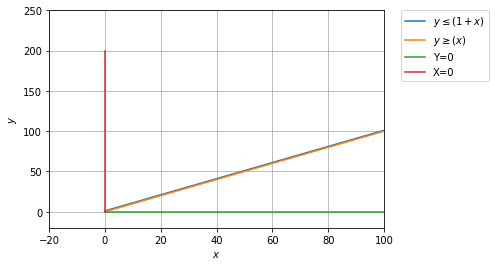
\includegraphics[width=\columnwidth]{solutions/sep/2/11/Figures/Figure.png}
\caption{Plot from python code }
\label{sep/2/11/fig}
\end{figure}
